\documentclass{msuposter}
\usepackage{lipsum}
\usepackage{tikz,wrapfig}
%% REQUIRED
\title{Using GANs to Generate Synthetic Data}
\author{Joseph Despres and Yunus Shariff}
\institute{Michigan State University}


%% SET COLUMN WIDTH
\newcommand{\colwidth}{0.3\linewidth}

\begin{document}
\begin{frame}{}
\begin{columns}[t]

\begin{column}{\colwidth}

\begin{block}{Introduction and Motivation}

This project aims to extend the Generative Adversarial Network (GAN) beyond image generation by using the framework to create synthetic data. The objective of any GAN is to train a Neural Network capable of generating additional copies indistinguishable from training data. This is accomplished by training two adjacent Neural Networks competing against one another. The first network, refered to as the Generator is tasked with converting Gaussian noise into a datapoint. The other, known as the Discriminator, aims to determine if that data point is real. The Discriminator, like a normal neural network, aims to maximize classification accuracy. The Generator aims to maximize the Discriminator's misclassifications \cite{NIPS2014_5ca3e9b1}. This area has progressed to the point where GANs are regularly generating images and videos fooling even the most observant humans. Applications for this technology have yet to be fully realized. This project explores a potential application generate additional samples of tabular data.

\end{block}

\begin{block}{Use Cases}

\begin{itemize}
	\item \textbf{Generate additional subjects in controlled experiments}
\end{itemize}

Although data are becoming more and more available, there is still a need to generate more. Big data sets are often collected by convince rather than deliberate experiment, procuring additional samples of randomized controlled trial is quite expensive. Additionally, Neural Networks are not as transparent statistical model making them natural complements. By extension, we propose a framework in which Neural Networks generate additional data and statistical models draw inferences. 

\begin{itemize}
	\item \textbf{Generate data to fit models where data are confidential}
\end{itemize}

Since these data are generated from another data set, confidentially and privacy is far less of a concern. This framework could be used to generate new samples from confidential data permitting models to be trained in a way that is compliant with regulatory standards, ethics, and respectful of privacy. Privacy concerns are not nearly as strong of a concern in computer-generated data, as these are merely data produced from learning the structure of the mechanism producing the data. 

\end{block}

\begin{block}{Method}

The challenge associated with training a GAN to generate synthetic data in a row in a data frame is several orders of magnitude smaller than a standard photo image. A Neural Network has no difficulty fitting it with enough hidden layers. The challenge is learning the structure of the data without overfitting. This is a balance between fitting the data so well it mimics the data seen and underfitting where it cannot generate. Therefore, the networks are very shallow by modern standards. 


\begin{figure}
  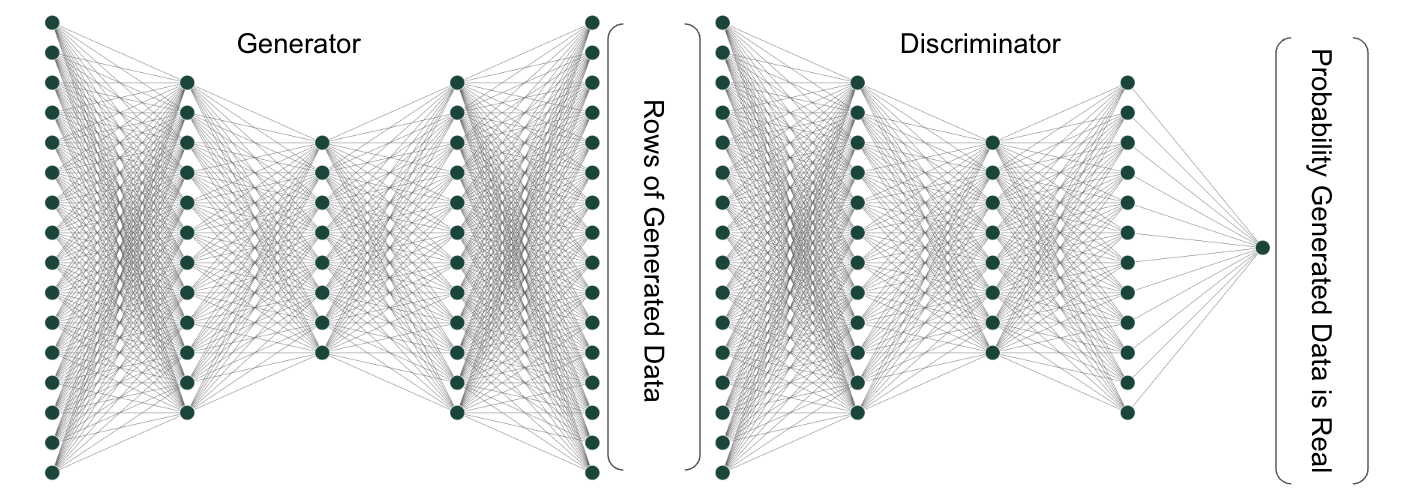
\includegraphics[width=\linewidth]{gan_diag.png}
    	\caption{\label{fig:my-label} Basic GAN Architecture Adapted to Generating Data}
\end{figure}

$$
\min_{G} \max_{D} V(D, G) = \mathop{\mathbb{E}}_{x \sim p_{data}} logD(x) + \mathop{\mathbb{E}}_{z \sim p_{z}(z)}log(1-D(G(z)))
$$

Using the method outlined by Hung \cite{hung} to generate additional data samples. These networks are small by today's standards with each layer being made up of less than 200 neurons and the network is made of less than 10 layers. Real and generated data are combined into a single data frame the discriminating network outputs a probability the data are real and fake given what it has learned from the training process. This is an iterative process and continues training until it converges to the point in which data are indistinguishable from real data. This training simply runs until all the numbers in the probability vector are 1.


\newpage 

\end{block}. 


\end{column}

%% COLUMN DIVIDE %%%%%%%%%%%%%%%%%%%%%%%%%%%%

\begin{column}{\colwidth}

\begin{block}{Experiment}

Developing this method data we use New York City Taxi from 2016\cite{nyc2016}. These data are far easier to verify than traditional experiments as there is a well defined plausible ranges for time and location, permitting simple filtering by heuristics. To generate longitude, latitude, and time for pick-up and drop-off of each fair, we assemble the GAN architecture. After that train the GAN on a subset of the data, then retrain adding data points. See Figure 2 for a minimal example of this process concatenating real and generated data then training the network until it converges to a solution.


\begin{figure}
  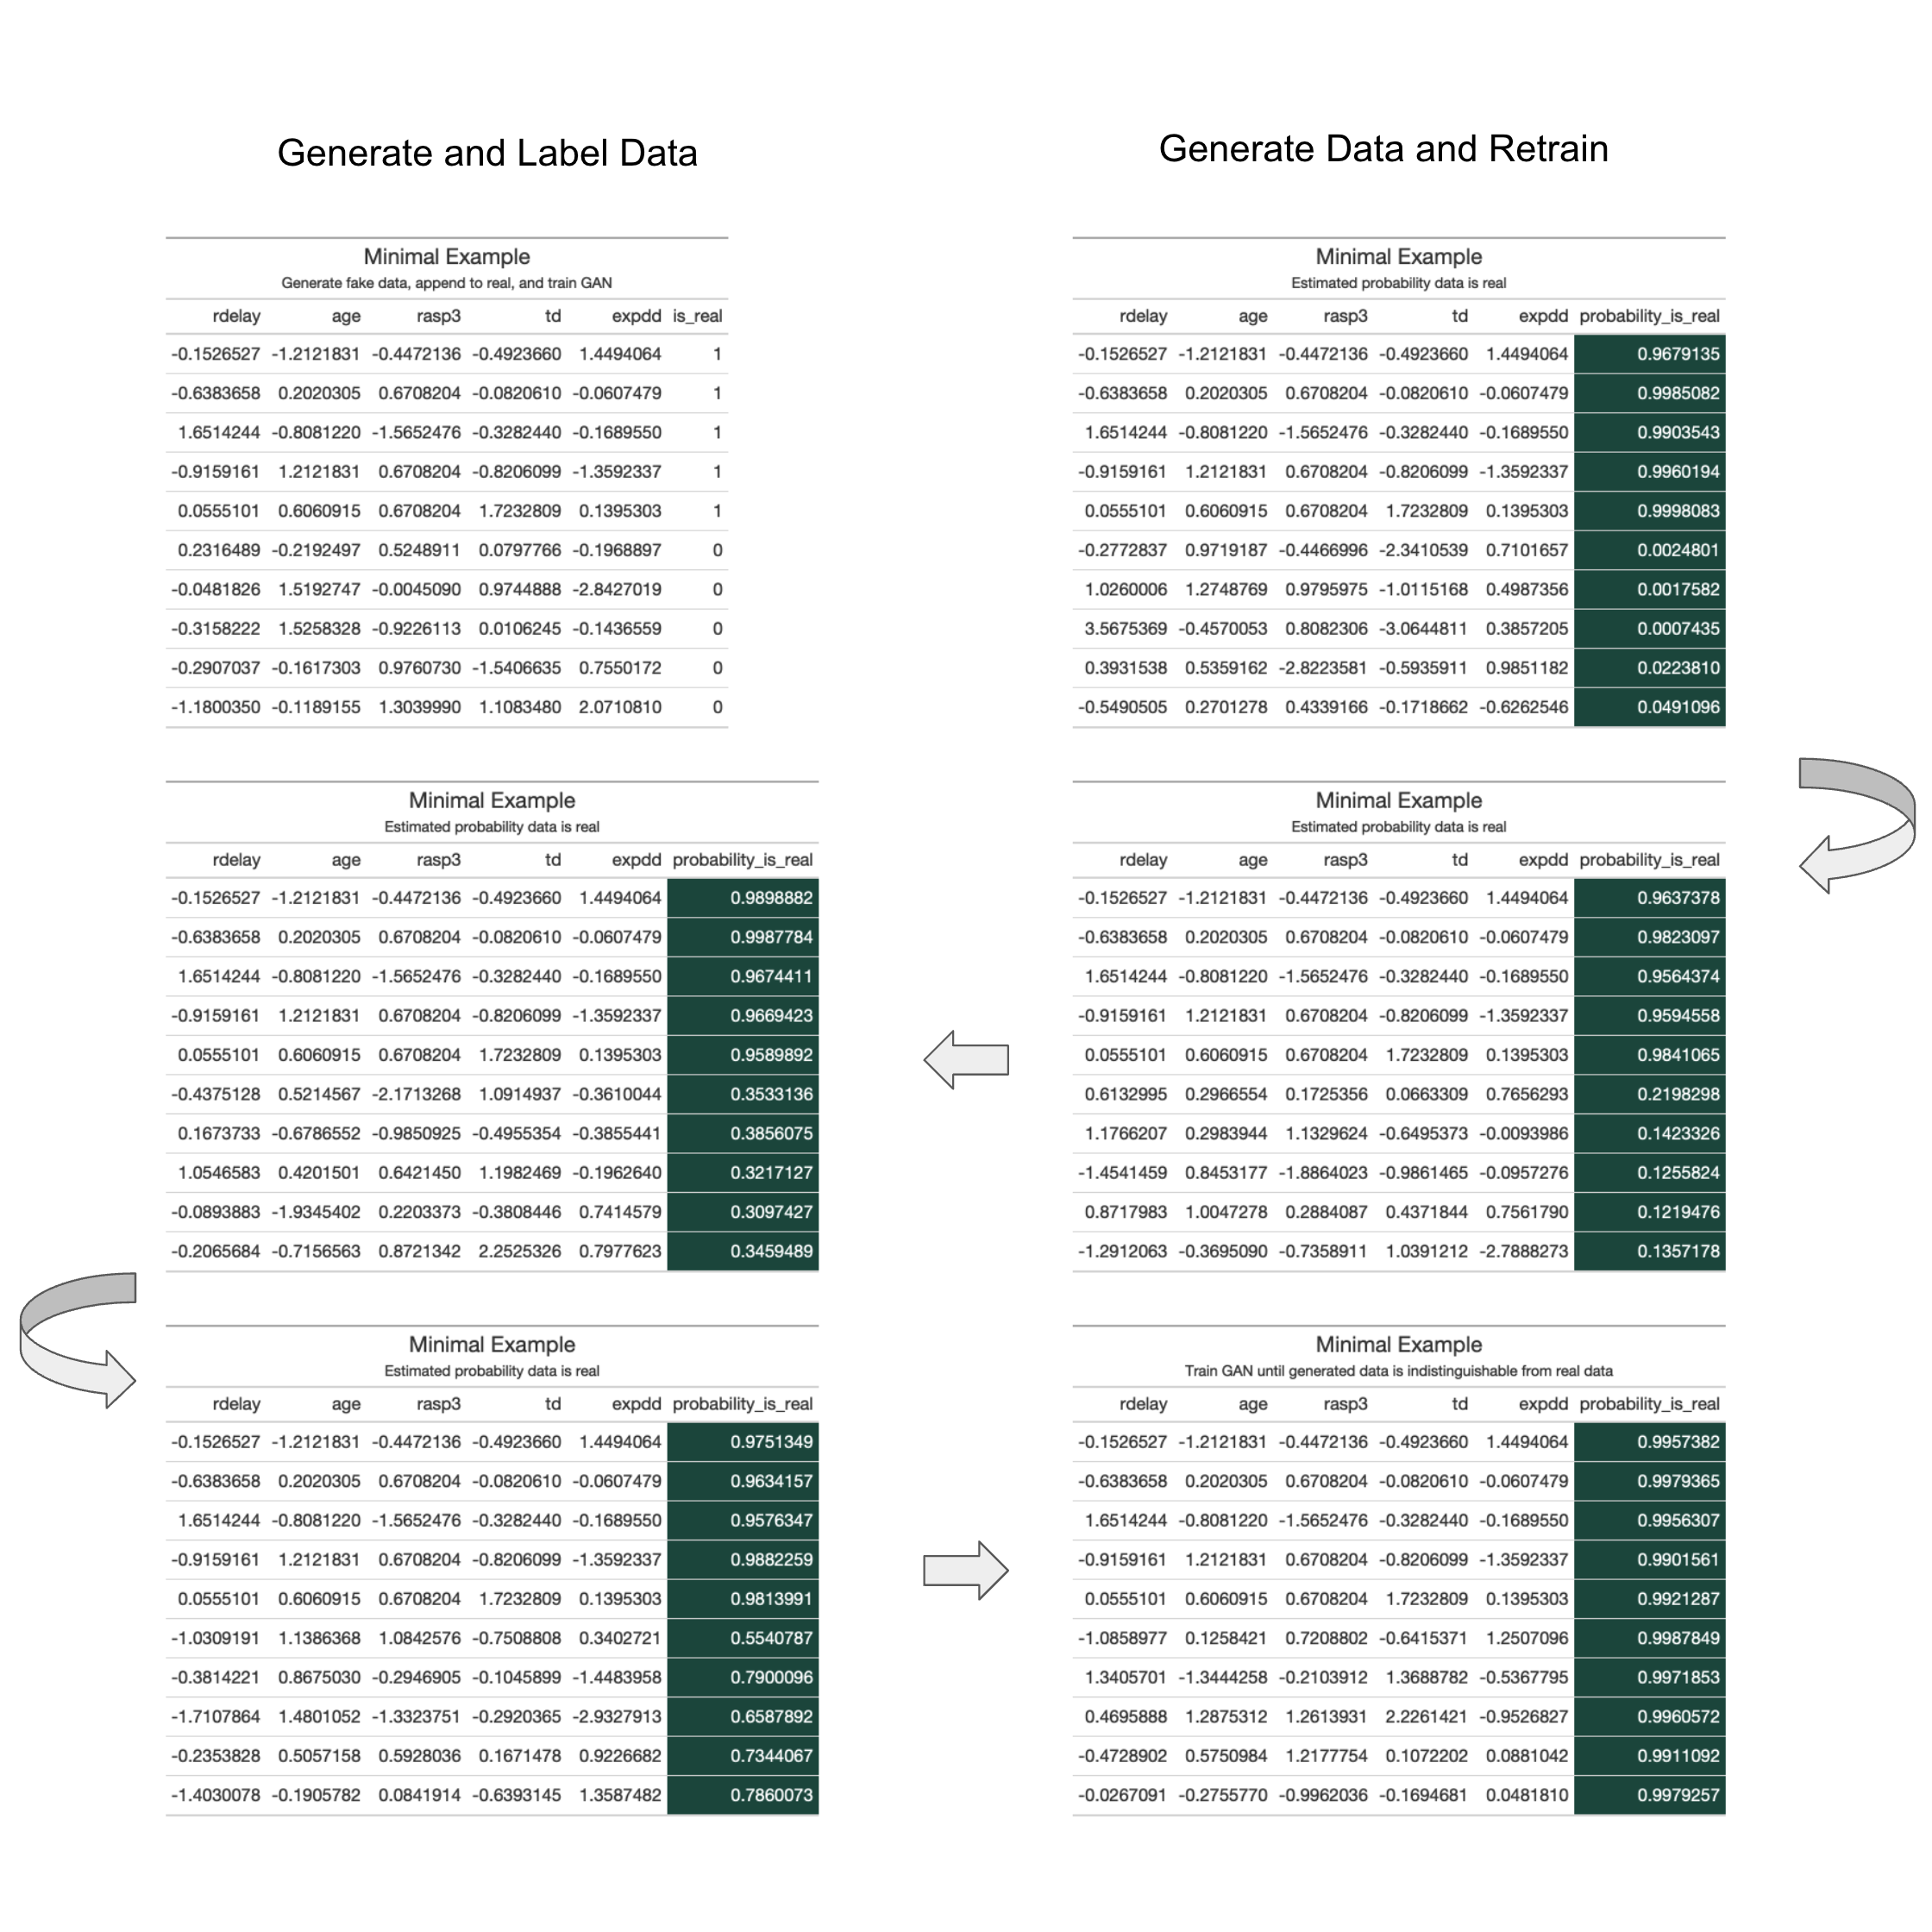
\includegraphics[width=\linewidth]{gan_conv.png}
      	\caption{\label{fig:my-label} GAN Generating Synthetic Data and Estimating Probability is Real}
\end{figure}

As shown in Figure 2, at first generated data are assigned a very low probability of being real. Note in Figure 3 the training process is cyclical, at times the generator is generating better samples than the discriminator is better at detecting generated samples. When this converges to 1, the discriminator is unable to distinguish between real and generated. 
\newline
\begin{figure}
  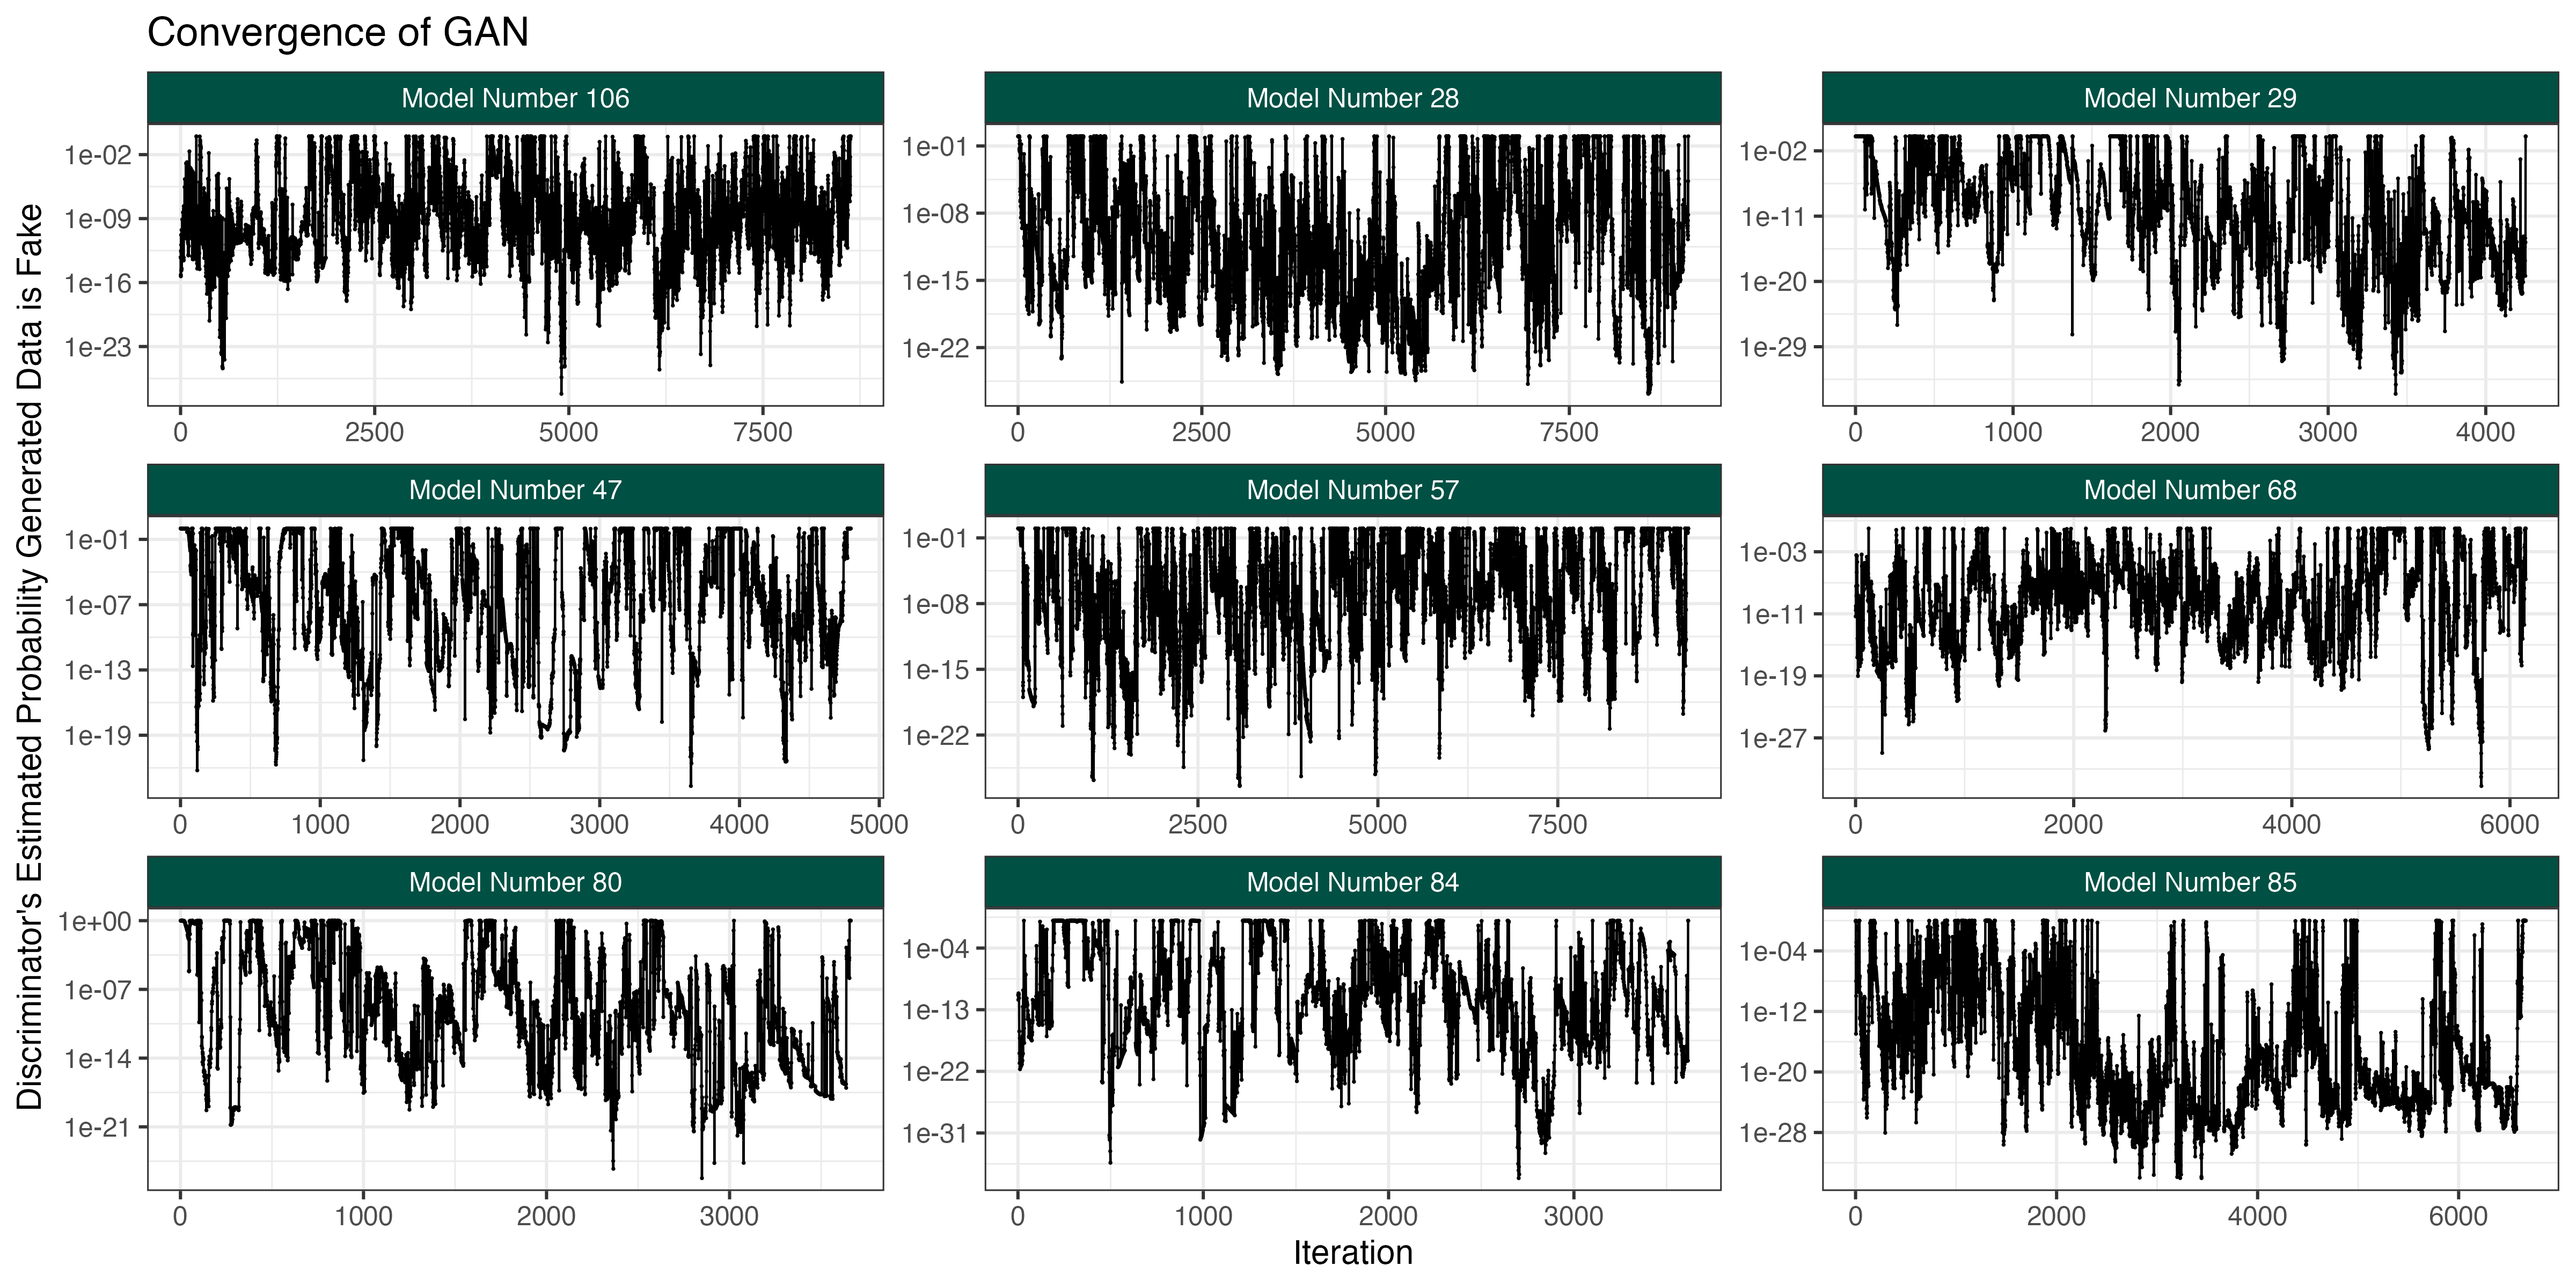
\includegraphics[width=\linewidth]{gan_converging.png}
  	\caption{\label{fig:my-label} New York City Taxi Data Real and Generated}
\end{figure}


\end{block}
\end{column}

%% COLUMN DIVIDE %%%%%%%%%%%%%%%%%%%%%%%%%%%%

\begin{column}{\colwidth}


\begin{block}{Results}

\begin{wrapfigure}{R}{0.5\textwidth}
\centering

\includegraphics[width=0.5\textwidth]{github.png}
\end{wrapfigure}
This method is able to generate synthetic taxi rides. Notice in Figure 4 generated taxi rides have a different structure from the ones in the dataset. These are mostly plausible, however this does showcase the need for verification. The data set contains a significant number of taxi rides going from the three airports to midtown. where the generated samples are going from midtown tout to the surrounding borrows. These generated samples, like most GANs, do require manual curation. Taxis should not be dropping people off in the middle of the river or on expressways. We can see that happening in a few of our generated samples. Manual inspection and curiation admittedly  limits the applications which is where this project falls short of our ambitions. 
\newline

\begin{figure}
  \includegraphics[width=\linewidth]{generated_map.png}
  	\caption{\label{fig:my-label} Probability data are real}
\end{figure} 


\end{block}


\begin{block}{Limitations and Further Study}

Despite the shallow architecture, this is quite expensive considering data generation methods such bootstrapping and boosting. The main cost is due to our GANs converging a whole network generating point regardless of input. Usually it is a plausible data point, but no guarantees. To remedy this, we retrain the GAN using a slightly different architecture often generating a random number of neurons, layers, and learning rates. This adds variation to the system by using a random Neural Network architecture. Additional study would involve data verification that does not involve a visual inspection. The need for visual inspection limits the type of applications this can be useful because most data will not be easy to verify. Also, using multiple datasets as well as adding convolutions to this network. This is the beginning of what could be a helpful method. 

\end{block}


\begin{block}{References}
\scriptsize
\bibliography{references}
\bibliographystyle{plain}
% \end{scriptsize}
\end{block}


%%%% end of references %%%%%%%%%%%%%%%%
\end{column}

\end{columns}
	\end{frame}
\end{document}


